% This document is used for Daya Bay MACRO PMT pressure test report


\documentclass{beamer}
\usepackage{graphicx}
\usepackage{gensymb} %for degree Celsius

\newcommand{\tabincell}[2]{\begin{tabular}{@{}#1@{}}#2\end{tabular}}

\usepackage{ragged2e}
\justifying

\usepackage{setspace}

\setbeamertemplate{navigation symbols}{}
\setbeamertemplate{footline}[page number]
\setbeamertemplate{caption}[numbered]
\setbeamerfont{caption}{size=\scriptsize}

\usetheme{default}
\logo{
\includegraphics[height=1cm]{Dyb_logo.png}}
\begin{document}
\title{Status of MACRO PMT pressure tests at SAB}
\author{Logan Lebanowski, Shih-Kai Lin}
\institute{University of Houston}
\date{2010 December 16}

\begin{frame}
\begin{center}
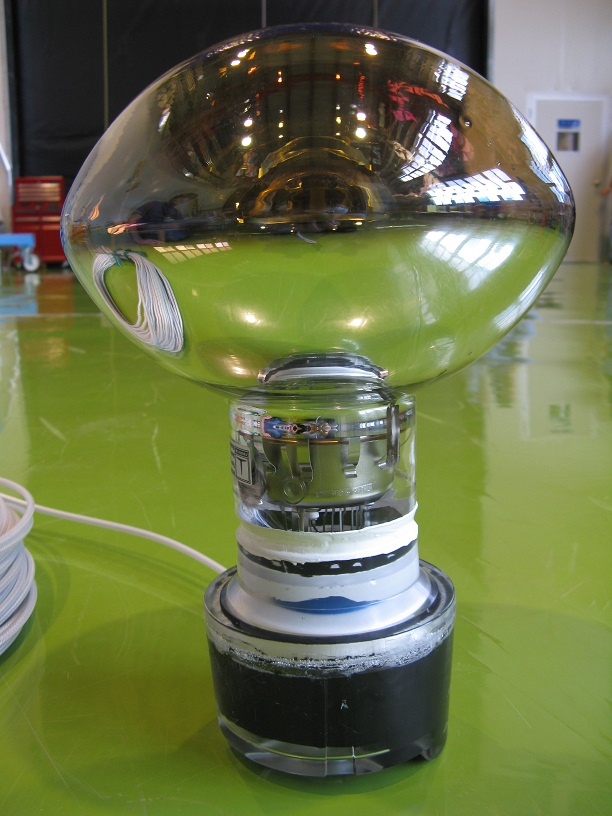
\includegraphics[height=4cm]{IMG_1048.jpg}
\end{center}
\titlepage
\end{frame}


\begin{frame}{overview}
	\begin{itemize}
		\item {\color{magenta}146} waterproof MACRO EMI PMT assemblies have been
pressure tested at the SAB. They had already passed performance tests at DGUT.
		\item We test about 10 PMTs per week (mid-August to December).
		\item For more information, see
			\textcolor{blue}{\href
			{http://dayabay.ihep.ac.cn/cgi-bin/DocDB/ShowDocument?docid=5373}{doc 5373}}.
	\end{itemize}
		\begin{center}
			\underline{We have passed 130(?) of all {\color{magenta}146} MACRO PMTs}\\
		\end{center}
	\begin{center}
		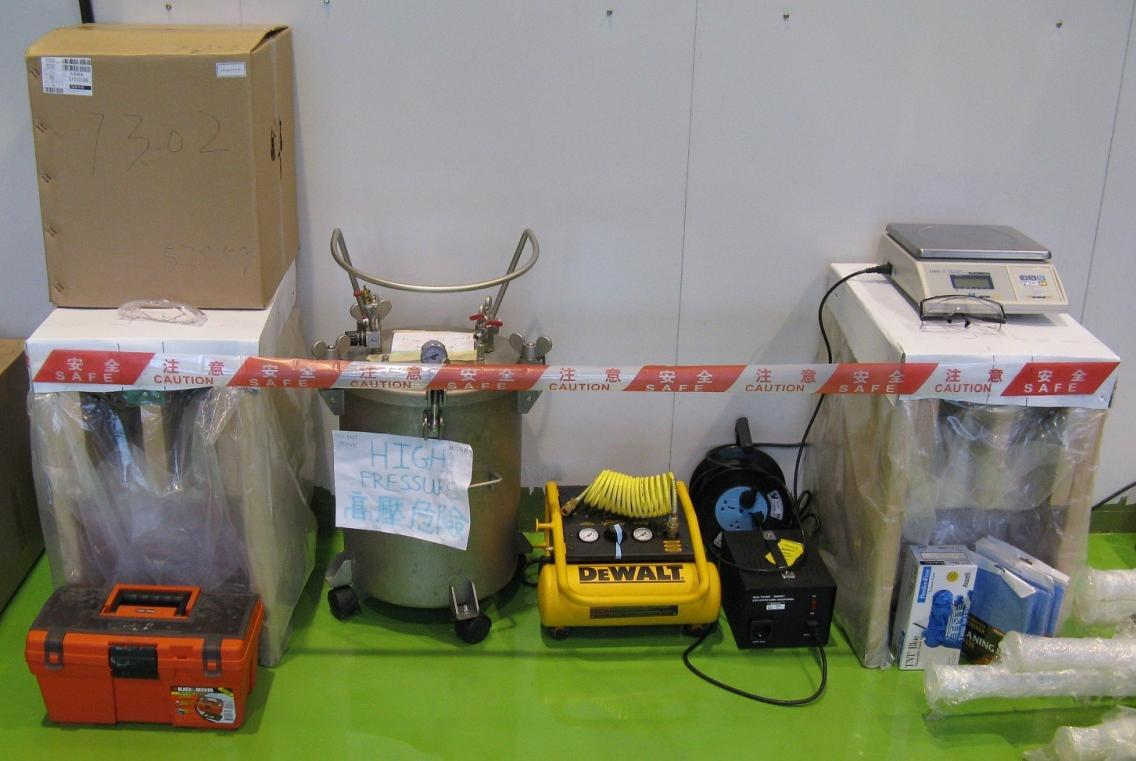
\includegraphics[height=4cm]{test_setup.jpeg}
	\end{center}
\end{frame}


\begin{frame}{pressure test results}
	\begin{center}
		\small
		8 PMTs were tested during the past week (December 9 - December 15).
\begin{table}
\begin{tabular}{c|c|c|c|c}
	SN & mass(g) & pressure (psig) & test time (h:m) & result \\
	\hline
	7005 & 577.5 & 12.2 & 14:58 & PASS$^1$ \\
	6944 & 556.5 & 12.1 & 8:12 & PASS$^1$ \\
	8921 & 567.0 & 12.0 & 15:38 & PASS$^1$ \\
	7418 & 606.0 & 12.1 & 7:39 & PASS$^1$ \\
	8724 & 629.5 & 12.1 & 15:22 & PASS$^1$ \\
	6960 & 569.5 & 12.0 & 7:18 & PASS$^1$ \\
	7229	& 643.0 & 12.0 & 20:23 & PASS$^1$ \\
	6572& 599.5 & 12.1 & 19:21 & PASS$^1$ \\
\end{tabular}
\begin{flushleft}
\scriptsize
	$^1$ Cable dry. No leaks or cracks.\\
\end{flushleft}
\end{table}
\end{center}
\end{frame}

\begin{frame}{signal test results}
	\setstretch{0.3}
	\small The operational capability of a PMT is verified after pressure testing:\\
	{\tiny The PMT is placed in a dark box, connected to a single channel
	decoupler box, and set to its 2E7 gain voltage, as recorded in the DGUT data.
	After tens of minutes, the count rate, rise time, and pulse height are
	recorded. We use a threshold of 3.00 mV, which is roughly 1/4 pe.
	}
	\begin{itemize}
		\item The last PMT carton is one with PMTs which didn't pass DGUT quality
		tests. Table~\ref{uqPMT} shows the reasons.
	\end{itemize}
	\setstretch{1}
	\setlength{\tabcolsep}{2pt}
	\scriptsize
%	\begin{center}
\begin{columns}[c] % the "c" option specifies center vertical alignment
\column{.55\textwidth} % column designated by a command
	\begin{tabular}{|c|c|c|c|c|}
		\hline
		\textbf{SN}&\textbf{Rate}&\textbf{DGUT}&\textbf{Rise}&
		\textbf{DGUT rise}\\
		&\textbf{(kHz)}&\textbf{rate (kHz)}&\textbf{time (ns)}&\textbf{time (ns)}\\
		\hline
		\hline
		7383   &4.8&0.47&4.7&5.0\\
		536   &9.5&0.49&3.7&4.0\\
		8216   &3.0&1.12&5.6&6.2\\
		9029   &6.0&0.42&5.7&6.2\\
		{\color{cyan}7418}  
&{\color{red}120-190$^\dagger$}&\color{red}257.24&4.8&3.2\\
		{\color{cyan}7005}  
&{\color{red}25-50$^\dagger$}&\color{red}28.26&4.9&13.0\\
		{\color{cyan}6944}   &&\color{red}14.94&&5.5\\
		{\color{cyan}8921}   &&\color{red}16.71&&3.7\\
		{\color{cyan}6572}   &&\color{red}12.46&&6.8\\
		{\color{cyan}6960}   &2.4&0.60&4.7&6.2\\
		{\color{cyan}8724}   &4.5&0.54&4.5&5.1\\
		{\color{cyan}7229}   &9.0&2.38&4.9&6.7\\
		\hline
	\end{tabular}
	\\ \color{red}$^\dagger$ These PMTs were tested for $\sim$20 hours. Their
	rates were unstable.
\column{.5\textwidth}
\centering
	\begin{table}
	\begin{tabular}{|c|c|}
		\hline
		\textbf{SN}&\textbf{reason of rejection}\\
		\hline
		{\color{cyan}7418}	&dark rate\\
		{\color{cyan}7005}	&dark rate\\
		{\color{cyan}6944}	&dark rate\\
		{\color{cyan}8921}	&dark rate\\
		{\color{cyan}6572}	&dark rate\\
		{\color{cyan}6960}	&after pulse ratio\\
		{\color{cyan}8724}	&after pulse ratio\\
		{\color{cyan}7229}	&after pulse ratio\\
		\hline
	\end{tabular}
	\caption{a carton of unqualified PMTs}
	\label{uqPMT}
	\end{table}
\end{columns}
\end{frame}

\begin{frame}{PMTs not passed so far}
\begin{columns}[c] % the "c" option specifies center vertical alignment
\column{.5\textwidth} % column designated by a command
	\footnotesize
		\begin{table}
			\begin{tabular}{|c|c|}
			\hline
			SN   & reason of \color{red}not pass \\
			\hline
			\color{cyan}7368 & water leaks into acrylic shell cap \\
			\color{cyan}7934 & water leaks into acrylic shell cap \\
			\color{cyan}7343 & water leaks into acrylic shell cap \\
			\color{cyan}9029 & water leaks into acrylic shell cap \\
			\color{cyan}7732 & water leaks into acrylic shell cap \\
			\color{cyan}7330	&	water leaks into acrylic shell cap \\
			\color{magenta}8727 & hole in cable jacket \\
			\color{magenta}8870 & hole in cable jacket \\
			\color{magenta}8377 & hole in cable jacket \\
			\color{magenta}7130 & hole in cable jacket \\
			7818	&	signal failure \\
			7418	&	high dark rate \\
			\hline
			\end{tabular}
		\caption{12 PMTs not passed}
		\end{table}
\column{.5\textwidth}
	\begin{itemize}
		\item We have begun repairing the 6 {\color{cyan}leaking} PMTs. Thanks to Weili for her work and instruction.
		\item We are preparing to repair the 4 PMTs with {\color{magenta}damaged
		cables}.
	\end{itemize}
	\footnotesize
		\begin{table}
			\begin{tabular}{|c|c|}
			\hline
			SN   & reason of \color{red}failure \\
			\hline
			8430 & broken \\
			6455 & broken \\
			7046 & imploded \\
			6545 & imploded \\
			\hline
			\end{tabular}
		\caption{4 PMTs failed}
		\end{table}
\end{columns}
\end{frame}

\begin{frame}{summary}
	\begin{itemize}
		\item All MACRO PMTs shipped from DGUT on August 10, 2010 have been
pressure tested.
		\item Repairs of not passed PMTs and the will be presented soon.
		\item A summary of test results will be given soon.
		\item A complete list of test results will be uploaded to \textcolor{blue}{\href
			{http://dayabay.ihep.ac.cn/cgi-bin/DocDB/ShowDocument?docid=4617}{doc 4617}}.
	\end{itemize}
\end{frame}

\end{document}
